\section{Личный вклад в развитие проекта}

В ходе разработки распределенной асинхронной системы обработки real-time
финансовых данных, я принял активное участие в формировании архитектуры проекта,
а также написал несколько сервисов, которые были важны для успешной работы
приложения.

Один из сервисов, который я написал --- это cmc-producer-ms. Этот сервис
отвечает за получение данных о криптовалюте с CoinMarketCap API и отправку их в
систему. Я также написал cmc-filter-ms, который отвечает за фильтрацию
полученных данных и отправку только необходимых данных в систему.

Одним из важных аспектов разработки приложения было обеспечение его
готовности к работе в условиях высокой нагрузки. Для этого я написал сбор метрик
с использованием Prometheus и Grafana (см Рис. \ref{grafana}).
Эти инструменты позволяют отслеживать
работу приложения в режиме реального времени и быстро реагировать на возможные
проблемы. Я также исправил докер образ с миграциями db-migrations, что позволило
быстро и легко обновлять базу данных при необходимости.

Одним из важных аспектов разработки приложения было обеспечение его
качества. Для этого я покрыл весь написанный мной код интеграционными и unit
тестами, что позволило быстро находить и исправлять возможные ошибки.
На рисунке \ref{tests} как раз можно увидеть пройденные тесты для сервиса cmc-filter-ms,
в котором реализовано тестирование маппинга сущностей и тестирование всего сервиса в целом.

\begin{figure}[h]
    \centering
    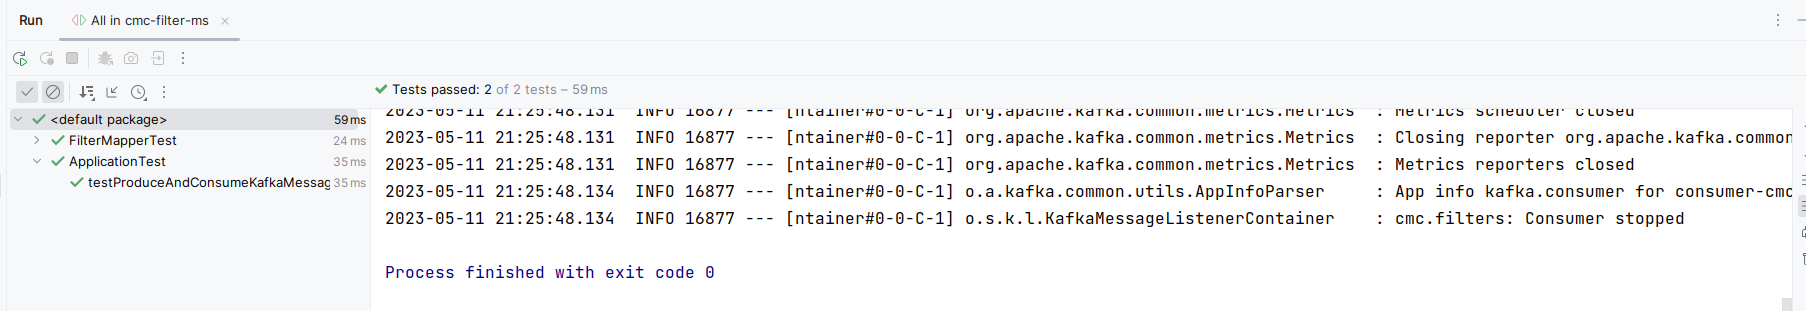
\includegraphics[width=0.95\linewidth]{passedtests.png}
    \caption{Изображение пройденных тестов сервиса cmc-filter-ms.}
    \label{tests}
\end{figure}

Мой личный вклад в развитие проекта был значительным. Я написал несколько
важных сервисов, которые были необходимы для успешной работы приложения. Я также
обеспечил готовность приложения к работе в условиях высокой нагрузки, написав
сбор метрик с использованием Prometheus и Grafana. Кроме того, я обеспечил
высокое качество кода, покрыв его интеграционными и unit тестами.